\documentclass{article}
\usepackage{mathtools}
\usepackage{xfrac}
\usepackage{amssymb}
\usepackage[utf8]{inputenc}

\begin{document}
% start
	\begin{eqnarray*}
		f(x)'=[x^{\sfrac{1}{2}}] + 1 = \frac{1}{2\sqrt{x}} + 1 \\
		\frac{1}{2}x^{-\sfrac{1}{2}}
	\end{eqnarray*}
	\begin{table}[h!]
  		\centering
  		\label{tab:table1}
  		\begin{tabular}{c | c c c}
    		t & ${x_t}$ & $f(x_t)$ & $f(x_t)'$\\
    		\hline
    		0 & 1 & -2 & 1.5\\
    		1 & 2.3333 & -0.1391 & 1.3273\\
    		2 & 2.4382 & -0.004 & \\
  		\end{tabular}
	\end{table}
	\[\tilde{x} = 2.4382 : |f(\tilde{x})|=0.0004 < 0.01 \]
	\[x_1=x_0 - \frac{f(x_0)}{f(x_0)'} = 1 - \frac{-2}{1,5} = 2.3333 \]
	\[x_2=x_1 - \frac{f(x_1)}{f(x_1)'} = 2.3333 - \frac{-0.1391}{1.3273}	= 2.4382
	\]
	\[\pmb{analytisch \ 0 \stackrel{!}{=} \sqrt{x}-4+x}\]
	\[\pmb{\curvearrowright \sqrt{x} = 4-x}\]
	\begin{align*}
	x = (4-x)^2=x^2-8x+16 \\
	x^2 -9x + 16 = 0 \\
	x_{1,2}=4.5\pm\sqrt{4.5^2-16} \\
	=4.5\pm 2.0616=
    \begin{cases}
		6.5616  \\
		2.4384 \in [0,4]
	\end{cases}	
	\end{align*}
	\section{Heron-Verfahren}
	Wurzel aus \begin{math} a > 0 \end{math} berechnen \\
	gesucht x mit \begin{math} f(x) = x^2 - a = 0 \end{math}
	\begin{align*}
	f'(x)&=2x \\
	x_{t+1}&=x_t-\frac{f(x_t)}{f'(x_t)} \\
	&=x_t-\frac{x_t^2-a}{2x_t} \\
	&=x_t-\frac{x_t}{2} \\
	&=(x_t+\frac{a}{x_t})\cdot\sfrac{1}{2}
	\end{align*}
	\section{Kreisfunktion und ihre Umkehrfunktion}	
		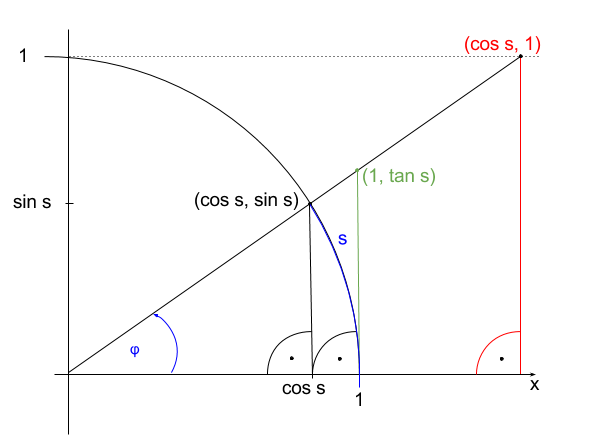
\includegraphics[scale=0.5]{png/circular_function.png}	
	\subsection{Kreisgleichung Radius R}
	\begin{align*}
		x^2+y^2&=r^2 \\
		hier \ r&=1 \ \ : \ \ x^2+y^2 = 1 \\
		\cos ^2 s + \sin ^2 &= 1 && \Leftarrow \text{(Pythagoras)} \\
	\end{align*}	
	\begin{flalign*}
		&\text{s Bogenlänge im Bogenmaß rad}&\\
		&\varphi \ Winkel \ im \ Winkelgrad \ deg \ [^\circ]&\\
		&Umfang \ eines \ Kreises \ mit \ Radius \ r&\\
	  	&U = 2\pi r \ (hier = 1)&\\
	  	&\frac{s}{\pi}=\frac{\varphi}{180^\circ}&\\
	\end{flalign*}
	\begin{align*}
		&\tan s=\frac{sin s}{\cos s} &\cot s =\frac{1}{\tan s}&
	\end{align*}
% stop
\end{document}